
%% bare_conf.tex
%% V1.3
%% 2007/01/11
%% by Michael Shell
%% See:
%% http://www.michaelshell.org/
%% for current contact information.
%%
%% This is a skeleton file demonstrating the use of IEEEtran.cls
%% (requires IEEEtran.cls version 1.7 or later) with an IEEE conference paper.
%%
%% Support sites:
%% http://www.michaelshell.org/tex/ieeetran/
%% http://www.ctan.org/tex-archive/macros/latex/contrib/IEEEtran/
%% and
%% http://www.ieee.org/


\documentclass[conference]{IEEEtran}
\usepackage{blindtext, graphicx}
 
% Início do código para entender português
%encoding
%--------------------------------------
\usepackage[utf8]{inputenc}
\usepackage[T1]{fontenc}
\usepackage{color}
\usepackage[]{algorithm2e}
\usepackage{tabularx}
\usepackage{booktabs}
%--------------------------------------
 
%Portuguese-specific commands
%--------------------------------------
\usepackage[portuguese]{babel}
%--------------------------------------
 
%Hyphenation rules
%--------------------------------------
\usepackage{hyphenat}
\hyphenation{mate-mática recu-perar}
%--------------------------------------
% FIM do código para entender português

% correct bad hyphenation here
\hyphenation{op-tical net-works semi-conduc-tor}

%para comentários em bloco
\usepackage{verbatim}

%outros pacotes
\usepackage{color}


\begin{document}
%
% paper title
% can use linebreaks \\ within to get better formatting as desired
\title{Reconhecimento Facial}


% author names and affiliations
% use a multiple column layout for up to three different
% affiliations
\author{\IEEEauthorblockN{Alex Santos Lopes}
\IEEEauthorblockA{Departamento de Computação\\
Instituto Federal da Bahia\\
Salvador, Brasil\\
Email: alexstlopes@ifba.edu.br}
}

% conference papers do not typically use \thanks and this command
% is locked out in conference mode. If really needed, such as for
% the acknowledgment of grants, issue a \IEEEoverridecommandlockouts
% after \documentclass

% for over three affiliations, or if they all won't fit within the width
% of the page, use this alternative format:
% 
%\author{\IEEEauthorblockN{Michael Shell\IEEEauthorrefmark{1},
%Homer Simpson\IEEEauthorrefmark{2},
%James Kirk\IEEEauthorrefmark{3}, 
%Montgomery Scott\IEEEauthorrefmark{3} and
%Eldon Tyrell\IEEEauthorrefmark{4}}
%\IEEEauthorblockA{\IEEEauthorrefmark{1}School of Electrical and Computer Engineering\\
%Georgia Institute of Technology,
%Atlanta, Georgia 30332--0250\\ Email: see http://www.michaelshell.org/contact.html}
%\IEEEauthorblockA{\IEEEauthorrefmark{2}Twentieth Century Fox, Springfield, USA\\
%Email: homer@thesimpsons.com}
%\IEEEauthorblockA{\IEEEauthorrefmark{3}Starfleet Academy, San Francisco, California 96678-2391\\
%Telephone: (800) 555--1212, Fax: (888) 555--1212}
%\IEEEauthorblockA{\IEEEauthorrefmark{4}Tyrell Inc., 123 Replicant Street, Los Angeles, California 90210--4321}}

% use for special paper notices
%\IEEEspecialpapernotice{(Invited Paper)}

% make the title area
\maketitle

% IEEEtran.cls defaults to using nonbold math in the Abstract.
% This preserves the distinction between vectors and scalars. However,
% if the journal you are submitting to favors bold math in the abstract,
% then you can use LaTeX's standard command \boldmath at the very start
% of the abstract to achieve this. Many IEEE journals frown on math
% in the abstract anyway.

% Note that keywords are not normally used for peerreview papers.


% For peer review papers, you can put extra information on the cover
% page as needed:
% \ifCLASSOPTIONpeerreview
% \begin{center} \bfseries EDICS Category: 3-BBND \end{center}
% \fi
%
% For peerreview papers, this IEEEtran command inserts a page break and
% creates the second title. It will be ignored for other modes.
\IEEEpeerreviewmaketitle


%Seções
\section{Introdução}\label{sec:introducao}

Muitos trabalhos buscam trazer novas maneiras ou aprimorar a tecnologia de identificação biométrica, surgindo assim novas maneiras fáceis e menos invasivas de identificação das pessoas pelas suas características físicas únicas (íris, voz, digital…) \cite{refer2}. E uma dessas tenta simular uma das formas mais naturais das pessoas reconhecerem umas às outras que seria pela identificação física, especificamente a facial.
Com o desenvolvimento de equipamentos computacionais cada vez mais rápidos \cite{refer5}, a utilização desse método tem sido muito utilizado ao passo que pesquisas na área tem buscado aprimoração, pela sua discrição e praticidade na identificação de pessoas \cite{refer1}.



\section{Referencial Bibliográfico}\label{sec:referencial-bibliografico}

Esta seção apresenta os principais assuntos relacionado a este trabalho. A subseção \ref{sec:solucao-desenvolvida} apresenta o método que será abordado para o problema apresentado na introdução. A subseção \ref{sec:viola-jones} Apresenta o funcionamento do algoritmo que será utilizado na solução. As subseções \ref{sec:haar-cascade}, \ref{sec:integral}, \ref{sec:ada-boost} e \ref{sec:cascade} detalha cada etapa presente no algoritmo Haar-Cascade (VIola-Jones).

\section{Solução Desenvolvida}\label{sec:solucao-desenvolvida}

Para a face ser rastreada deve considerar as condições do ambiente, ruídos, variação de iluminação, expressões faciais, imagem de fundo, orientação da cabeça, obstrução da face ou sobreposição de faces.
As técnicas mais citadas para realizar a detecção de faces são: casamento de padrões que consiste na detecção por meio de comparações com formas geométricas, modelos estatísticos, modelos baseado em redes neurais, modelos baseados em tons de pele e o
Viola; Jones \cite{refer3}.


\section{Viola-Jones}\label{sec:viola-jones}

Paul Viola e Michael Jones propuseram em 2001 uma abordagem para
detecção de objetos em imagens que se baseia em três conceitos: integral de imagem,
treinamento de classificadores usando boosting e o uso de classificadores em cascata.
Esse algoritmo é capaz de identificar qualquer objeto, mas o seu intuito é utilizar na identificação de faces. Sua maior vantagem é a precisão em encontrar imagens correspondente e sua rapidez de execução \cite{refer4}.

\section{Haar-Cascade}\label{sec:haar-cascade}

Método cascade há um conjunto de imagens, as que contém as características que se deseja extrair (imagens positivas) e as que não tem correspondência com o que deseja (imagens negativas). Um exemplo seria com a detecção facial. Haveria um conjunto de imagens de faces, positivas, e outras que não fossem faces, negativas.

%\begin{comment}

\begin{figure}[ht]
\centering
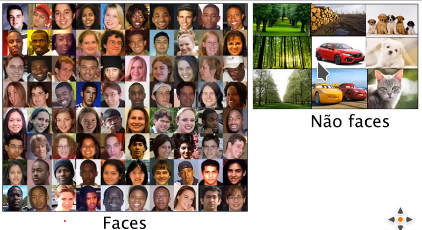
\includegraphics[width=8cm]{images/cascade.png}
\caption{Exemplos de faces usadas pelo cascade}
\label{fig:cascade}
\end{figure}

%\end{comment}

Logo após um treinamento de imagens é feito com o algoritmo AdaBoost. E por seguinte é selecionado os melhores conjuntos de características. A característica é dada pela soma dos pixels que se situam dentro dos retângulos brancos e são subtraídos da soma dos pixels em retângulos em cor cinza segundo Viola e Jones (2001). Então, esse resultado irá representar o valor encontrado pela característica para determinada região \cite{refer4}.

Ao tentar identificar um rosto seja em uma foto ou um vídeo, é feito a busca pixel por pixel até encontrar características que sejam correspondente. 

A partir da integral de imagem é possível identificar padrões utilizando características Haar-like, que são máscaras retangulares nas quais os valores dos pixels de uma região são subtraídos dos valores dos pixels de outra região, representando uma diferença de intensidade luminosa entre áreas da imagem. 
O algoritmo é dividido em três partes:
A criação da imagem integral, a representação da imagem em um espaço de características baseados nos filtros de Haar.

Montagem de um classificador de aprendizado Boosting chamado de AdaBoost, capaz de selecionar as características relevantes.

Criação de uma estrutura em árvore, chamada cascata de classificadores.

\section{Integral}\label{sec:integral}

A integral de imagem, também conhecida como tabela de soma de áreas, é um
algoritmo, proposto por Frank Crow em 1984, que permite avaliar eficientemente a soma
dos valores dos pixels (intensidade dos níveis de cinza) de uma área retangular em uma
sub-região da imagem \cite{refer1}.

\section{Ada Boost}\label{sec:ada-boost}

O AdaBoost é derivado de Adaptative Boosting, o algoritmo de boosting, é um método de aprendizado de máquina que utiliza a combinação de vários classificadores fracos (weak learners – de hipóteses fracas) para obter uma classificação forte (de hipótese forte). O Boosting é utilizado tanto para selecionar um conjunto de características como para treinar o classificador.
Durante o treinamento, os atributos retangulares (características) são localizados e analisados, verificando se são úteis ao classificador. Quando as características de Haar são aplicadas em uma imagem, são examinados os contrastes naturais proporcionados pelas características da face, considerando suas relações de espaço.

\section{Cascade}\label{sec:cascade}

A última etapa consiste em combinar classificadores fortes em cascata de modo a
processar eficientemente regiões da imagem em busca de um padrão. Cada estágio na cascata aplica um classificador mais específico e complexo do que o anterior, de modo que o algoritmo rejeite rapidamente regiões que sejam muito distintas da característica procurada e termine o processo de procura neste caso, evitando que os estágios posteriores sejam executados desnecessariamente. Isso faz com que muitos dos cenários e panos de fundo sejam descartados nos primeiros estágios e apenas faces e outros objetos semelhantes a faces sejam analisados mais exaustivamente \cite{refer4}. 

%\begin{comment}
\begin{figure}[ht]
\centering
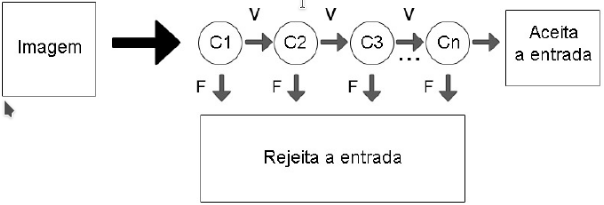
\includegraphics[width=8cm]{images/haar-cascade.png}
\caption{Seleção das imagens}
\label{fig:haar cascade}
\end{figure}

%\end{comment}

\section{Conclusão}\label{sec:conclusao}

Na presente pesquisa foi apresentado o potencia da tecnologia de reconhecimento de faces e seu processamento utilizando o algoritmo de Viola-Jones.  Nota-se assim
que a técnica possibilita a detecção facial de por meio de computação visual. A detecção, ainda, apresenta alguns desafios a serem superados, principalmente quando é realizada em ambientes não controlados.




% Can use something like this to put references on a page
% by themselves when using endfloat and the captionsoff option.
\ifCLASSOPTIONcaptionsoff
  \newpage
\fi


% biography section

\bibliography{references.bib}
\bibliographystyle{IEEEtran}


% that's all folks
\end{document}


